\section{How many different tours?}
\begin{frame}{Count the tours: 2 cities, then 3}
\princ{COUNTING / PATTERN}
Fix the start at city 1. Count the closed tours that visit every city once.\\[6pt]
\textbf{2 cities:} \NToursTwo\ \hfill $\Rightarrow$ \textbf{\NCountTwo} tour.\\[6pt]
\textbf{3 cities:} \NToursThree\ \hfill $\Rightarrow$ \textbf{\NCountThree} tours.\\[6pt]
\predict{How many tours for 4 cities? Write down a guess before the next slide.}
\note{Build this on the board, not from the slide. For two cities there is one tour: go to the other and come back. For three, after 1 you can choose 2 or 3, and then the last is forced. Notice that 1-2-3-1 and 1-3-2-1 are different tours because this table is asymmetric. Ask for guesses for four cities. Expected guesses: 3, 4, 6, 8. Collect them without comment.}
\end{frame}

\begin{frame}{4 cities}
\princ{COUNTING / PATTERN}
All the orders of cities 2, 3, 4 after the start:\\[6pt]
\NToursFour\\[6pt]
\see{\textbf{\NCountFour} tours.}
\vspace{6pt}
\begin{itemize}
\item 3 choices for the first stop, then 2 for the second, then 1 for the last.
\end{itemize}
\note{Let students call out the list while you write it; the code that made this list is in the last section. Compare with their guesses. Point at the pattern: three choices, then two, then one. Do not give the formula yet. Question: what would five cities look like? Expected: four choices, then three, two, one.}
\end{frame}

\begin{frame}{The reasoning: choices shrink by one each step}
\princ{COUNTING / PATTERN}
For $n$ cities with the start fixed, there are $n-1$ cities left to order:
\begin{center}
\begin{tabular}{@{}lccccc@{}}
slot & 2nd stop & 3rd & 4th & 5th & 6th\\
choices (6 cities) & 5 & 4 & 3 & 2 & 1
\end{tabular}
\end{center}
Multiply: $5\times4\times3\times2\times1=5!$ \quad $\Rightarrow$ \quad $(n-1)!$ tours.\\[4pt]
\see{\NCountFive\ tours for 5 cities, \NCountSix\ tours for 6.}
\note{The reasoning is the point, not the numbers. Each time you pick, one fewer city remains. The product of a shrinking list is a factorial. Ask: why does the first slot have n minus 1 choices and not n? Expected: because the start city is already used. Check: 5 times 4 is 20, times 3 is 60, times 2 is 120, times 1 is 120.}
\end{frame}

\begin{frame}{The pattern}
\princ{COUNTING / PATTERN}
\begin{center}
\begin{tabular}{c|ccccc}
cities $n$ & 2 & 3 & 4 & 5 & 6\\\hline
tours $(n-1)!$ & \NCountTwo & \NCountThree & \NCountFour & \NCountFive & \NCountSix
\end{tabular}
\end{center}
\vspace{4pt}
\predict{What is the next number, for 7 cities?}
\begin{itemize}
\item Each step multiplies by the next whole number: $\times2,\ \times3,\ \times4,\ \times5$.
\end{itemize}
\note{Let the room say the pattern: each new city multiplies the count by n minus 1. Ask for 7 cities; it is 6 times 120, so 720. (That is the computer's number too: the code section asserts the formula for n from 2 to 6.) Say: the numbers look small now. Keep that feeling for two slides.}
\end{frame}

\begin{frame}{Which counting convention? Say it once}
\princ{COUNTING / PATTERN}
\begin{itemize}
\item \textbf{Our convention:} start fixed at city 1, direction matters. Count $=(n-1)!$.
\item Do not fix the start: list all $n!$ orders, but each tour appears $n$ times (rotations), and you get the same $(n-1)!$ tours. For 6 cities: \NFactSix\ listings, \NCountSix\ tours.
\item Ignore direction (a two-way street): a tour and its reverse are the same, so halve: $(n-1)!/2$, which is \NHalfSix\ for 6 cities.
\end{itemize}
\see{Our table is asymmetric, so a tour and its reverse are different tours. \textbf{No halving.}}
\note{Say this once and move on. If you do not fix the start, you can list six factorial, seven hundred twenty, ordered lists of six cities, but they describe the same tours six times each. If the street were two-way and the distances symmetric, a tour and its reverse would have the same total, and you could halve the count. Our table is one-way on purpose, so we do not. Jeremy's convention is the first bullet. Ask: which convention does the word asymmetric rule out? Expected: halving.}
\end{frame}

\begin{frame}{Plot it (linear)}
\princ{COUNTING / PATTERN}
\begin{center}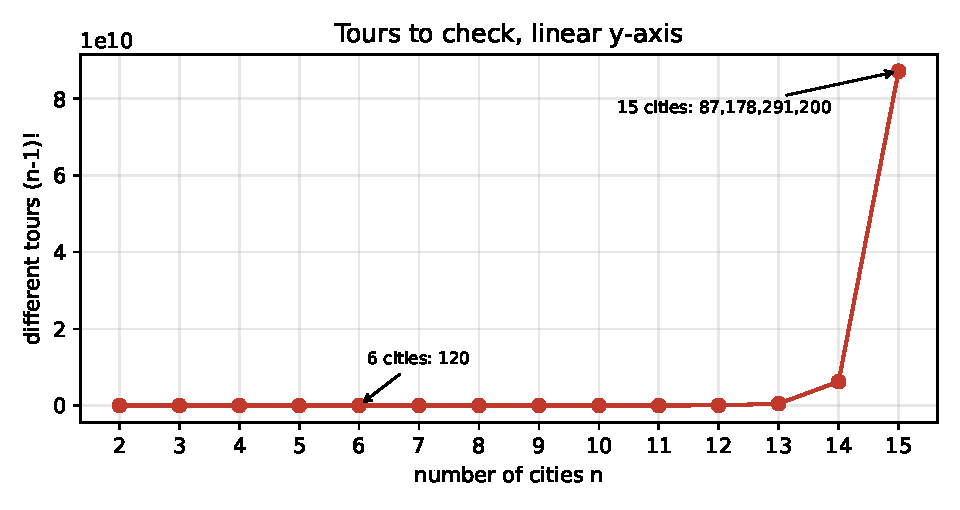
\includegraphics[height=5.3cm]{../figures/tour_count_linear.pdf}\end{center}
\see{the curve is flat for a few cities, then it shoots off the page.}
\note{Drawn by \texttt{scripts/make\_figure.py}. Ask what they see. Expected: almost nothing happens until about ten, then it explodes. The linear picture hides how fast it grows at the start, which is why we need the log version next.}
\end{frame}

\begin{frame}{Plot it (log)}
\princ{COUNTING / PATTERN}
\begin{center}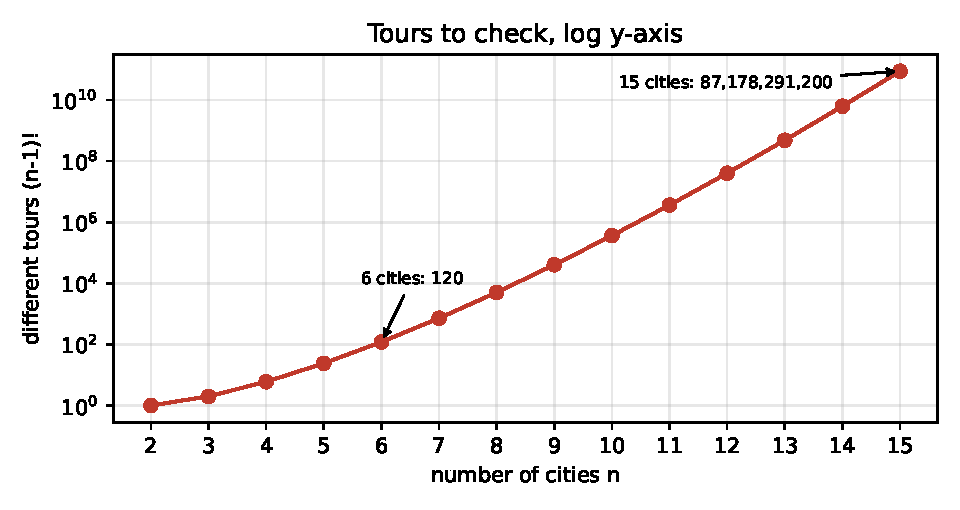
\includegraphics[height=5.3cm]{../figures/tour_count_log.pdf}\end{center}
\see{each step up the axis is a factor of ten; the line still bends upward.}
\note{On a log axis an exponential becomes a straight line; this bends upward, so it grows faster than exponential. Ask them to read the 15-city point. Do not rush it. Ten cities is \NCountOneZero\ tours; fifteen is \NCountOneFive.}
\end{frame}

\begin{frame}{What the curve means for brute force}
\princ{COUNTING / PATTERN}
\begin{itemize}
\item 6 cities: \textbf{\NCountSix} tours. A laptop does that instantly.
\item 10 cities: \NCountOneZero\ tours.
\item 15 cities: \textbf{\NCountOneFive} tours (about \NCountOneFiveBillions{} billion).
\end{itemize}
\vspace{4pt}
\see{at one million tours per second, 15 cities takes about \NHoursAtMillion\ hours. (The speed is an assumption.)}
\note{Trying every tour is correct, because it checks everything, and hopeless for large n. Correct and not practical are different things. At one million tours per second, a made-up but generous speed, fifteen cities takes about a day. Ask: what do we do instead of brute force? Expected: smarter methods, or accept a good-enough answer such as greedy. That is why people care about the shortest-path problem.}
\end{frame}
